% ----------------------------------------------------------
\chapter{Fundamentação Teórica}\label{cap:Fundamentação teórica}
% ----------------------------------------------------------
Neste capítulo, são apresentados os conceitos e teorias que fundamentam o desenvolvimento do braço robótico 4R e seu sistema de controle. A base teórica é dividida em três pilares principais: primeiramente, o ecossistema ROS 2, que atua como o \textit{middleware} de comunicação e orquestração dos processos; em seguida, a modelagem cinemática, essencial para a tradução de coordenadas cartesianas em movimentos angulares; e, por fim, os protocolos de comunicação CAN, que estabelecem o elo entre a lógica de software e o hardware físico das juntas.

\section{O ECOSSISTEMA ROS 2}
O \textit{Robot Operating System 2} (ROS 2) consiste em um ecossistema de software de código aberto (\textit{open-source}) amplamente consolidado tanto na comunidade acadêmica quanto na indústria de automação para o desenvolvimento e controle de sistemas robóticos complexos. Descaracterizando-se como um sistema operacional convencional, o ROS 2 atua como um \textit{middleware} robótico, fornecendo uma infraestrutura de comunicação estruturada sobre o padrão DDS (\textit{Data Distribution Service}). Essa arquitetura viabiliza a construção de aplicações distribuídas, interconectando de forma robusta e escalável os diversos componentes de software e hardware de um robô.

A topologia de comunicação do ROS 2 fundamenta-se em uma rede de computação modular, cujos pilares essenciais de interação são divididos em nós, tópicos e serviços, conforme detalhado a seguir.

\subsection{Nodes (Nós)}
Os \textit{Nodes} representam as unidades modulares de processamento de dados e execução de algoritmos dentro do ecossistema. Cada nó constitui um processo independente e especializado, encarregado de executar uma tarefa computacional restrita e bem definida, como a aquisição de dados de um sensor de visão computacional, o cálculo cinemático de um manipulador robótico composto por juntas revolutivas, ou a modulação de sinais de tensão para o acionamento de \textit{drivers} de potência. A descentralização em múltiplos nós operando concomitantemente confere ao sistema tolerância a falhas e alto grau de reaproveitamento de código.

\subsection{ Topics (Tópicos)}
Os Tópicos estabelecem canais de comunicação unidirecionais e contínuos, estruturados sob o modelo arquitetural de \textbf{publicação e inscrição} (\textit{publish/subscribe}). Nesse arranjo, um nó produtor de informação (\textit{publisher}) envia mensagens contendo dados estruturados a um barramento específico (por exemplo, as coordenadas cartesianas do efetuador de um braço articulado). De forma assíncrona, um ou mais nós consumidores (\textit{subscribers}) inscrevem-se no referido tópico para receber o fluxo de dados em tempo real, tornando este mecanismo ideal para variáveis de estado de alta frequência, como odometria e leituras de sensores industriais.

\subsection{Services (Serviços)}
Diferente da natureza contínua dos tópicos, os Serviços operam com base em um acoplamento temporário sob o paradigma de \textbf{requisição e resposta} (\textit{request/response}). Este modelo de comunicação síncrona ou assíncrona pontual subdivide-se em:
\begin{itemize}
    \item \textbf{Cliente:} O nó que demanda uma ação ou um processamento de dados específico;
    \item \textbf{Servidor:} O nó que recebe a requisição, executa a rotina matemática ou lógica correspondente e retorna uma resposta estruturada de confirmação ou os dados processados ao cliente.
\end{itemize}
Este mecanismo é estritamente empregado para operações discretas, transições de estados globais do sistema ou configurações de parâmetros que exijam validação imediata de execução.

\subsection{Visualização Gráfica via rqt graph}
Para fins de diagnóstico, depuração e análise topológica da rede de comunicação, o ecossistema disponibiliza a ferramenta computacional \textit{rqt graph}. Trata-se de uma interface gráfica de introspecção que mapeia dinamicamente o grafo de computação do sistema em tempo real. A ferramenta renderiza os nós ativos como vértices e os fluxos de dados (tópicos e serviços) como arestas direcionadas, permitindo ao projetista inspecionar visualmente as interconexões da arquitetura robótica, validar a integridade dos canais de comunicação e rastrear anomalias estruturais.

A Figura \ref{fig:rqt_graph} exemplifica de forma abstrata a representação gráfica gerada por essa ferramenta de diagnóstico em um sistema robótico em operação.

\begin{figure}[htbp]
    \centering
    \caption{Representação gráfica do grafo de computação via \textit{rqt\_graph}.}
    \label{fig:rqt_graph}
    \vspace{1cm} % Espaço vertical reservado para a inserção posterior do diagrama geométrico/imagem
    
    % Nota para o autor: Substitua a caixa abaixo pela inclusão real da sua imagem.
    % Exemplo: \includegraphics[width=0.85\textwidth]{meu_diagrama_rqt.png}
    
    \begin{center}
        \boxed{
            \begin{minipage}{0.85\textwidth}
                \vspace{4cm}
                \centering
                \textit{[Espaço reservado para inserção do diagrama do rqt\_graph]}
                \vspace{4cm}
            \end{minipage}
        }
    \end{center}
    
    \vspace{0.3cm}
    \small Fonte: Elaborado pelo autor (2026).
\end{figure}

\section{Robôs Manipuladores}%tipos
O termo "robô"  originou-se em 1920, introduzido pelo dramaturgo tcheco Karel Čapek na peça Rossum's Universal Robots, derivando da palavra robota, que significa "trabalhador". Ao longo do tempo, a nomenclatura passou a ser atribuída a praticamente qualquer dispositivo mecânico que opere com certo grau de autonomia sob controle computacional, englobando desde teleoperadores e drones até veículos subaquáticos e autônomos. Contudo, apesar dessa vasta aplicabilidade tecnológica, o escopo do texto restringe-se à análise conceitual e prática de duas categorias específicas: os manipuladores industriais e os robôs móveis. Nesse contexto, a estrutura e a classificação geral de diferentes tipos de robôs, incluindo as categorias de foco e exemplos fora do escopo, podem ser visualizadas na Figura \ref{fig:Robos tipos}.\cite{spong2005robot}.

\begin{figure}[htbp]
    \centering
    \caption{Tipos de robôs.}
    \label{fig:Robos tipos}
    \vspace{0.2cm}
    
    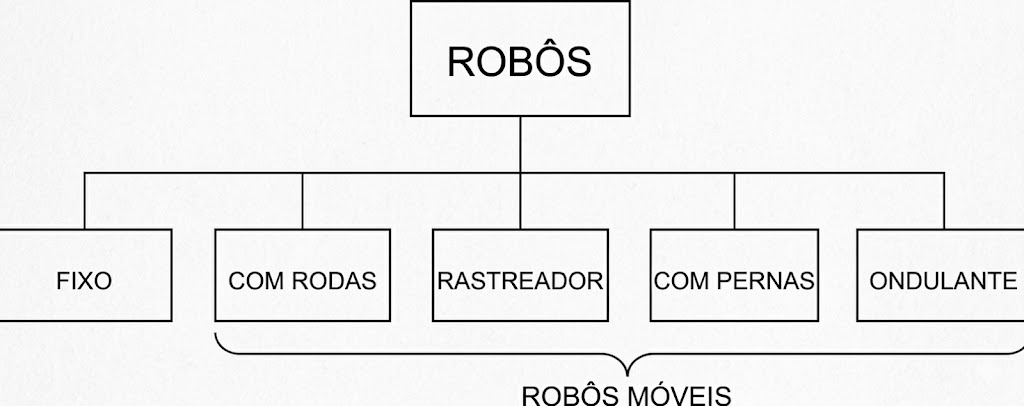
\includegraphics[width=0.8\textwidth]{template_eca_ufsc_abnt/figuras/Robo_tipo.png}
    
    \vspace{0.3cm}
    \small Fonte: Adaptado de \cite{siciliano2009robotics}.
\end{figure}


Um sistema robótico é fundamentalmente constituído por quatro subsistemas interdependentes 
que integram percepção e ação: o mecânico, o de atuação, o sensorial e o de controle. 
O sistema mecânico compõe a estrutura física do robô, sendo subdividido em aparatos de 
locomoção e de manipulação, conforme ilustrado na Figura~\ref{fig:componentes_robotica}. 
A movimentação dessa estrutura é viabilizada pelo sistema de atuação, o qual engloba 
servomotores, acionamentos e transmissões responsáveis pelo controle cinemático e dinâmico. 
Para interagir com o meio, o sistema sensorial coleta dados do estado interno e externo por 
meio de sensores proprioceptivos e exteroceptivos, realizando o condicionamento de sinais e 
o processamento de informações. Por fim, o sistema de controle atua como o núcleo inteligente, 
aplicando princípios de retroalimentação (\textit{feedback}), inteligência artificial e 
planejamento de tarefas para coordenar as ações motoras a partir dos dados percebidos, 
respeitando as restrições físicas e ambientais impostas.

\begin{figure}[htbp]
    \centering
    \caption{Componentes de um sistema robótico.}
    \label{fig:componentes_robotica}
    \vspace{0.2cm}
    
    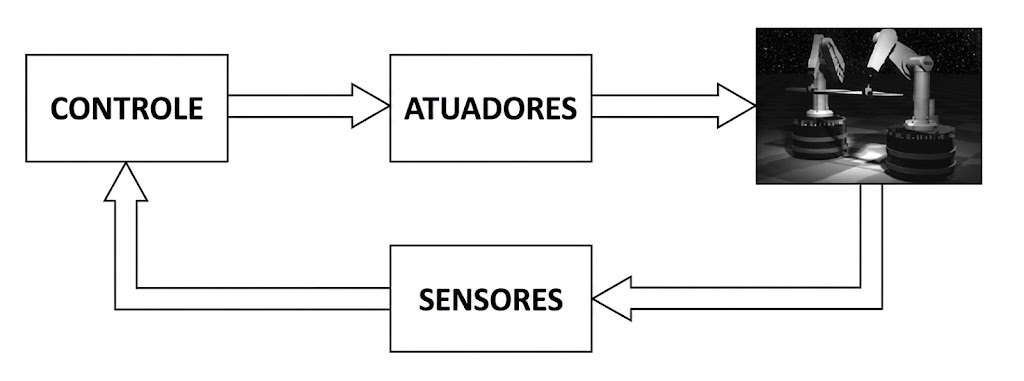
\includegraphics[width=0.8\textwidth]{template_eca_ufsc_abnt/figuras/componentes_robotica.png}
    
    \vspace{0.3cm}
    \small Fonte: Adaptado de \cite{siciliano2009robotics}.
\end{figure}

\subsection{Notação} 
A 
\begin{figure}[htb]
	\caption{\label{fig:Angulos de EUler}Notação de Euler.}
	\begin{center}
		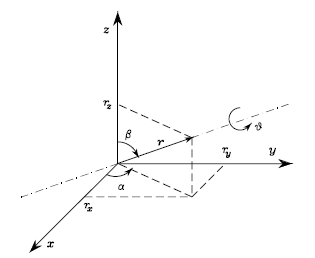
\includegraphics{template_eca_ufsc_abnt/figuras/Notação.png}
	\end{center}
	\fonte{\cite{spong2005robot}.}
\end{figure}

\subsection{Graus de Liberdade e Espaço de Configuração}
A configuração de um manipulador é a especificação completa da localização de cada ponto do robô. O conjunto de todas as configurações possíveis que o equipamento pode assumir é chamado de espaço de configuração. Como os elos do manipulador são estruturas perfeitamente rígidas conectadas a uma base fixa, a posição geométrica de qualquer ponto do robô pode ser inferida de forma direta assim que os valores exatos de cada variável de junta sejam conhecidos. Por conta disso, uma configuração é matematicamente representada por um vetor contendo os valores correspondentes a essas variáveis.\cite{spong2005robot}.

Nesse contexto, um objeto possui $n$ graus de liberdade (DOF) se a sua configuração puder ser especificada por um número mínimo de $n$ parâmetros independentes. Para um manipulador robótico padrão, é o número de juntas que determina a quantidade de graus de liberdade do sistema. Essas juntas são tipicamente classificadas em revolutas, que permitem a rotação relativa entre elos adjacentes, ou prismáticas, que viabilizam um movimento relativo linear, conforme ilustrado na Figura \ref{fig:JuntasRP} . Um objeto rígido e livre no espaço tridimensional, por exemplo, necessita de exatos seis graus de liberdade para ter a sua pose completamente definida: três parâmetros dedicados ao posicionamento espacial (translação) e três parâmetros para a sua orientação. Consequentemente, o número de graus de liberdade de um robô equivale à dimensão exata do seu espaço de configuração \cite{spong2005robot}.

\begin{figure}[htb]
	\caption{\label{fig:JuntasRP}Tipos de Juntas.}
	\begin{center}
		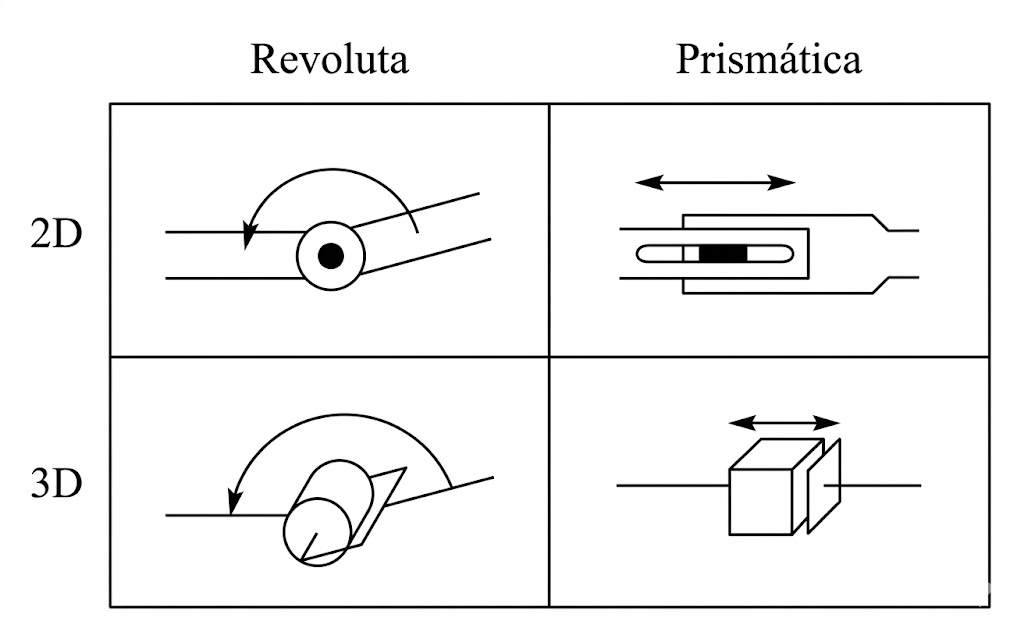
\includegraphics[width=0.8\textwidth]{template_eca_ufsc_abnt/figuras/JuntasRP.png}
	\end{center}
	\fonte{ Adaptado de \cite{spong2005robot}.}
\end{figure}



\subsection{Representação da posição em função da mudança de orientação}


\subsection{Rotações Elementares}


\subsection{Composição de Matrizes de Rotação}


\subsection{Ângulos de Euler }

\subsection{Convenção de Denavit-Hartenberg}

\subsection{Inversa Cinemática}

\section{Protocolo CAN}
\subsection{CPR CAN V2}




